\documentclass[12pt]{article}

\usepackage[utf8]{inputenc}
\usepackage[margin=1in]{geometry}
\renewcommand{\baselinestretch}{1}
\usepackage{indentfirst}

\usepackage{amsmath, amssymb}

\usepackage{graphicx}
\usepackage{float}
\graphicspath{{./figs/}}

\begin{document}

\begin{center}\begin{LARGE}
\textbf{Assignment 4: Results/Description}
\end{LARGE}\end{center}

\section*{Problem 1}

\subsection*{(a)}



\begin{figure}[ht]
    \centering
    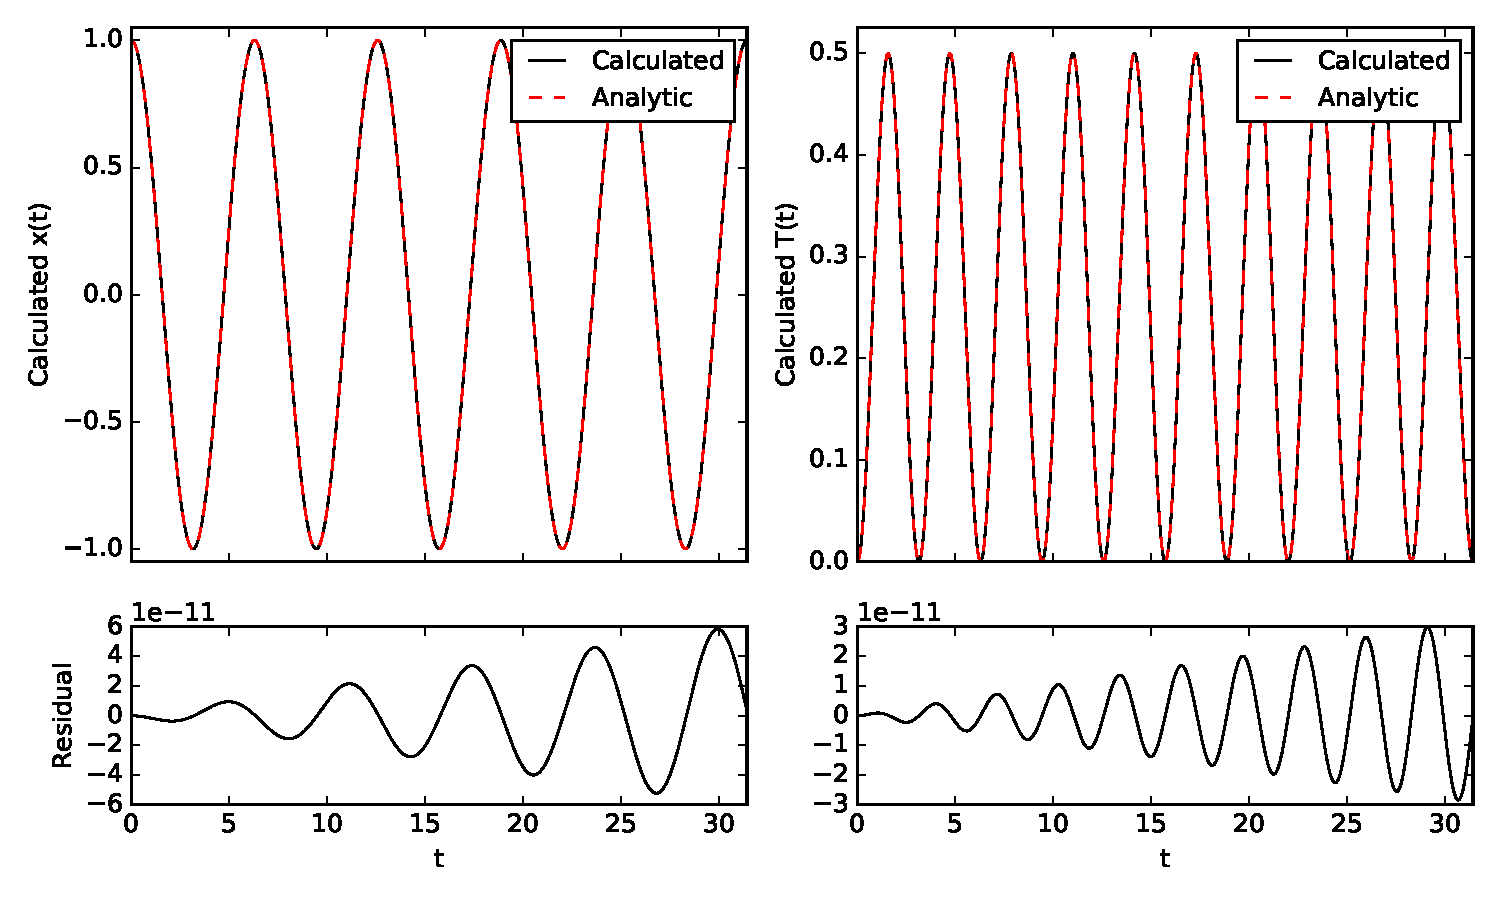
\includegraphics[width=0.9\textwidth]{odeint}
    \caption{Solution using the ODEInt (BS) method.}
    \label{fig:odeint}
\end{figure}

\subsection*{(b)}



\begin{figure}[ht]
    \centering
    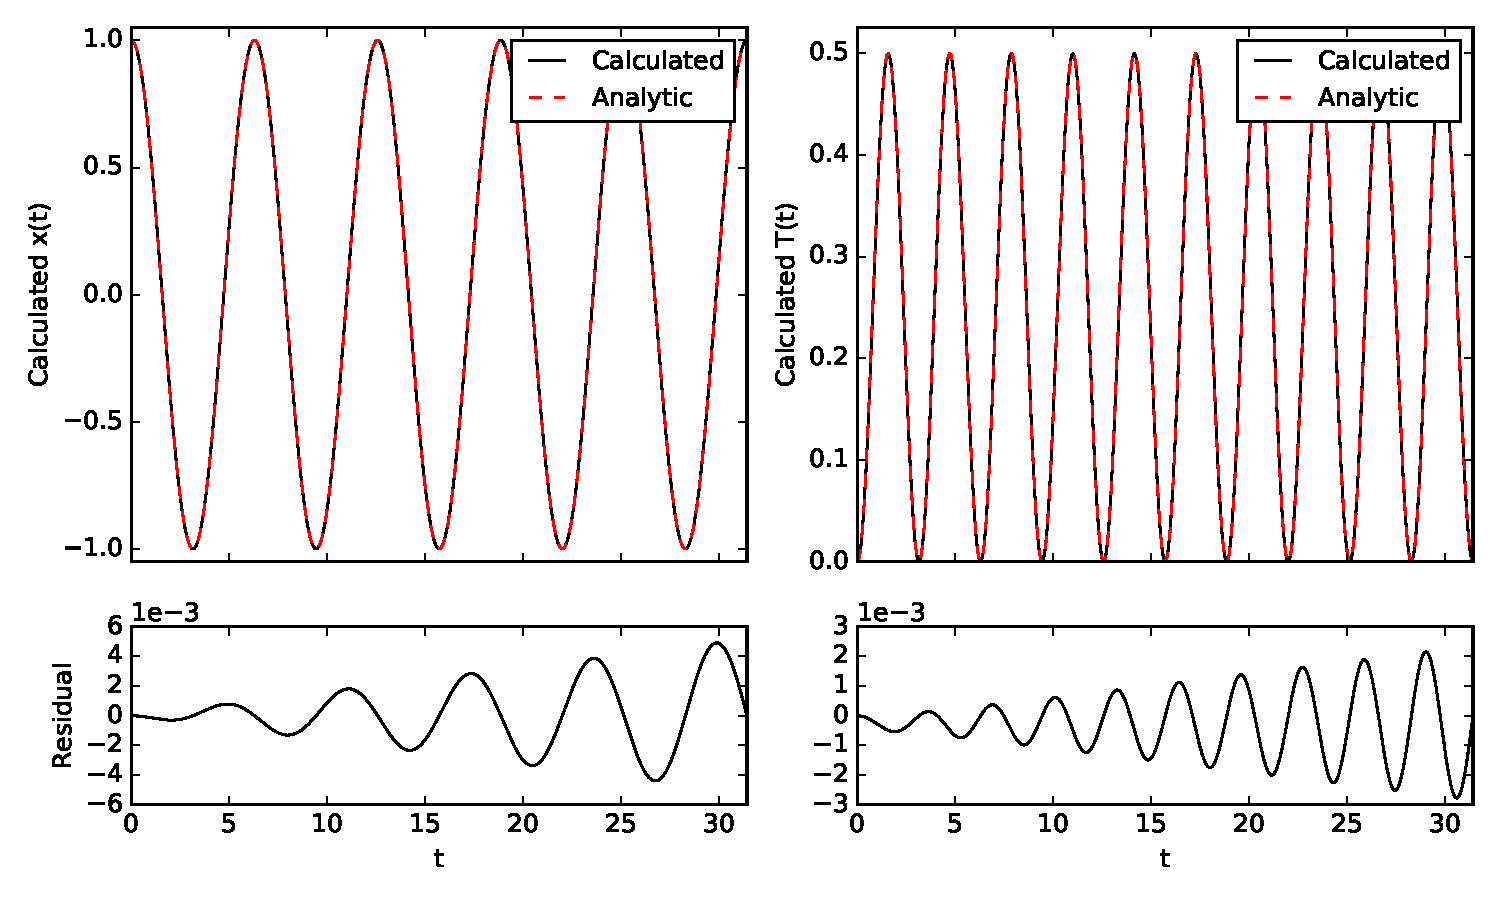
\includegraphics[width=0.9\textwidth]{leapfrog}
    \caption{Solution using the Leapfrog method.}
    \label{fig:leapfrog}
\end{figure}

\subsection*{(c)}



\begin{figure}[ht]
    \centering
    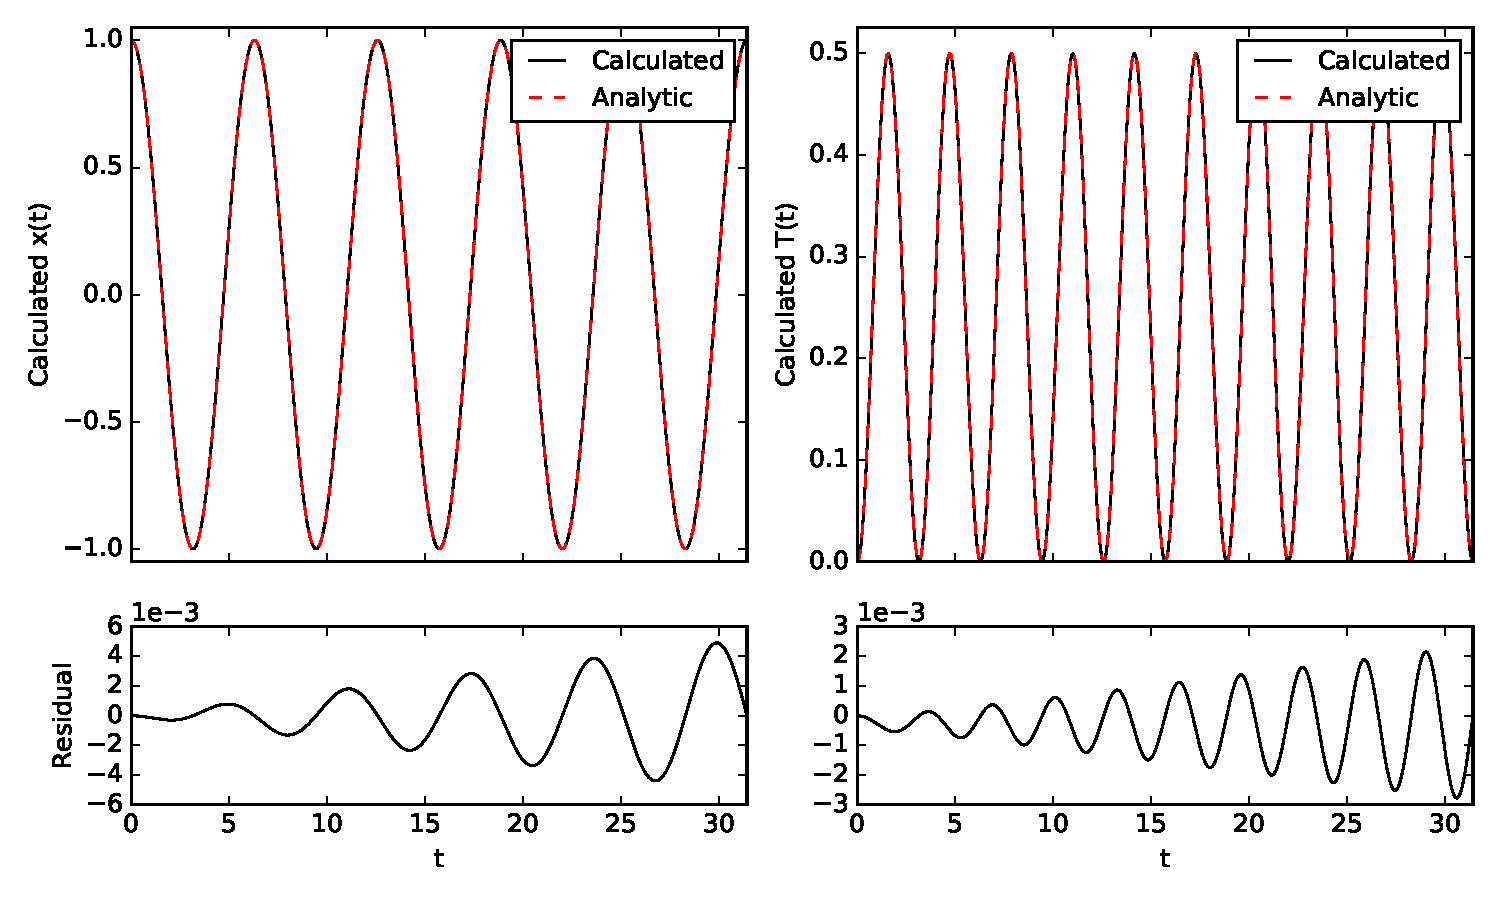
\includegraphics[width=0.9\textwidth]{velverlet}
    \caption{Solution using the Velocity Verlet method.}
    \label{fig:velverlet}
\end{figure}

\subsection*{(d)}




\end{document}
